%% Additional packages

\documentclass[a4paper, 12pt]{article}
\usepackage{fontspec}
\usepackage{graphicx}
\usepackage{hyperref}
\usepackage[margin=1.5cm]{geometry}
\usepackage{amsmath}
\usepackage[polish]{babel}

%% Title

\title{\textbf{Symulacja ruchu ludzi w centrum handlowym}}
\author{Paweł Kłeczek \and Kajetan Rzepecki}
\date{2012-11-09}


%% Text starts here:
\begin{document}

    \vspace{\fill}
    \maketitle
    \vspace{\fill}
    \thispagestyle{empty}

\newpage
    \setcounter{page}{1}
    \setcounter{tocdepth}{3}
    \tableofcontents

\newpage
    \section{Wprowadzenie}
    \label{sec:intro}

\noindent
Celem wykonywanego projektu jest stworzenie modelu oraz symulacja ruchu ludzi w centrum handlowym w oparciu m.in. o model \hyperref[refs:social-distances-1]{\textit{Social Distances}}.

Modelowanie ruchu dużych grup ludzi w środowisku zorganizowanym jest problemem złożonym i wymaga wykorzystania równie złożonych algorytmów celem dokładnego przybliżenia rzeczywistych zachowań. Dobrym podejściem jest dekompozycja problemu modelowania złożonego zjawiska na mniejsze, łatwiejsze do rozwiązania podproblemy, którymi zajmują się osobne, dobrze zdefiniowane i wyspecjalizowane algorytmy i ponowne połączenie wyników ich działania w spójną całość - metoda \textit{Divide and Conquer}.

    \begin{figure}[h!]
        \centering
        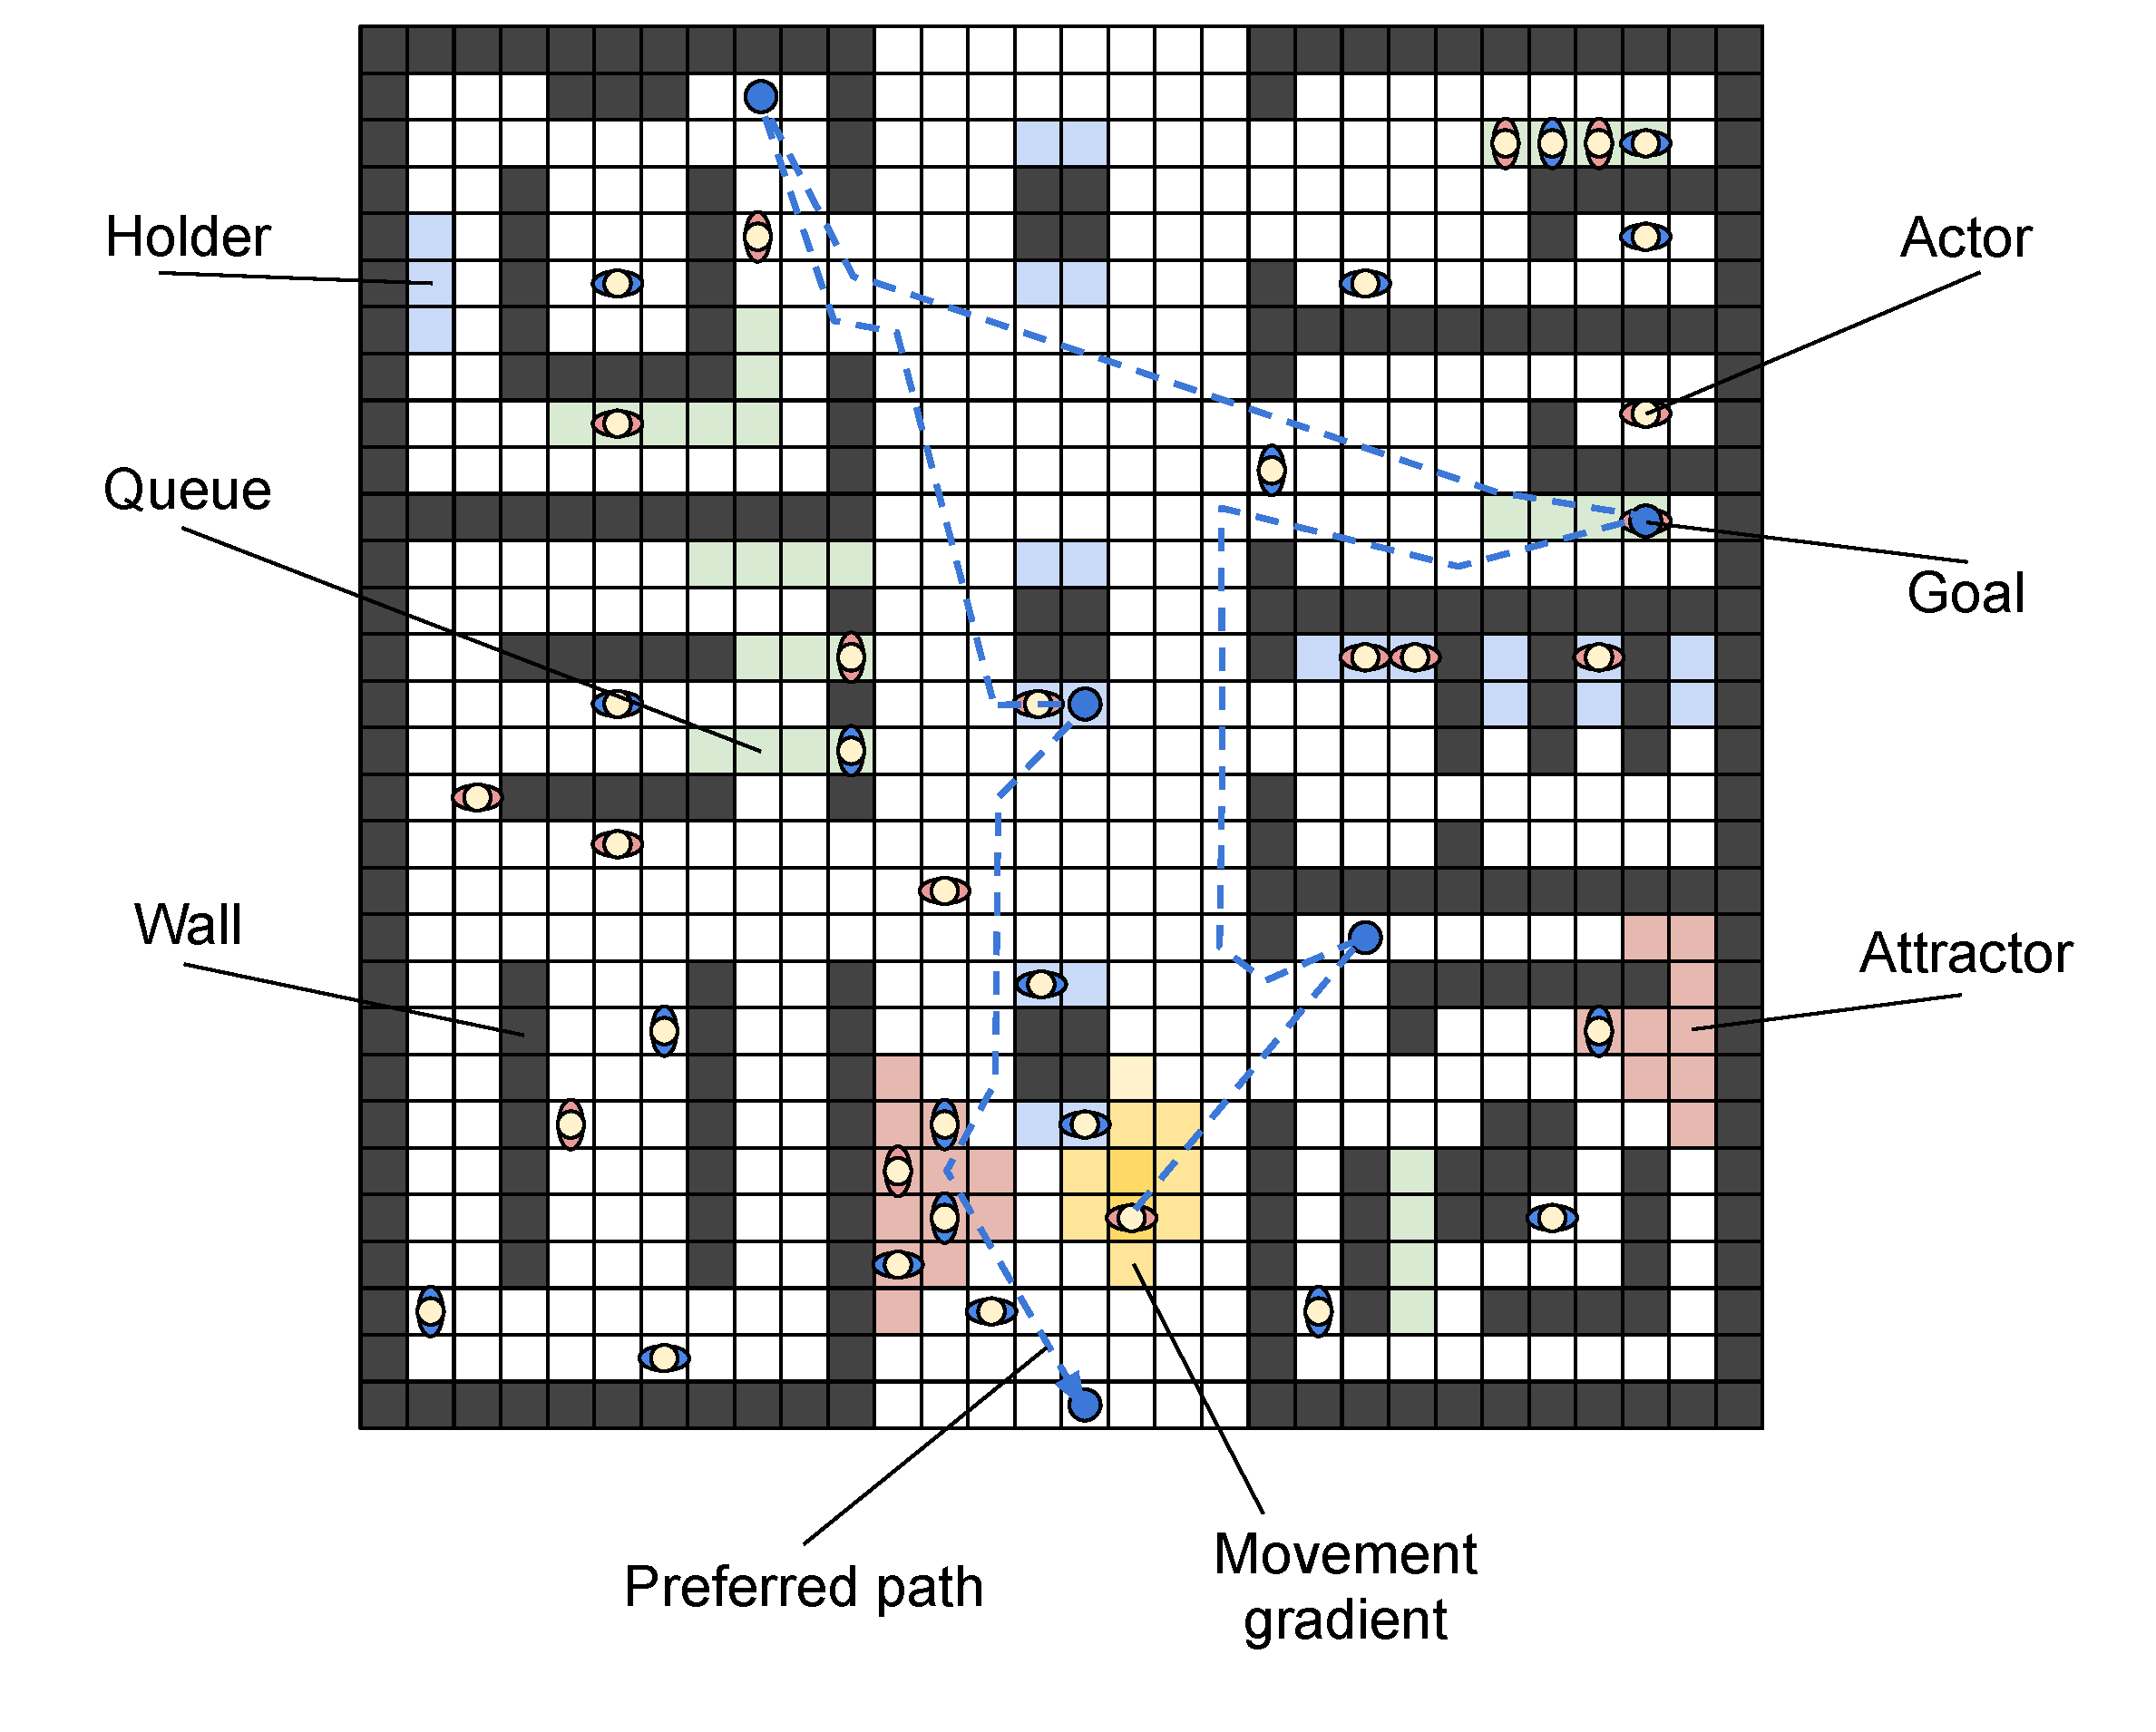
\includegraphics[scale=0.3]{./img/Overview.pdf}
        \caption{Przykładowa dekompozycja problemu modelowania ruchu ludzi w centrum handlowym.}
        \label{fig:decomp}
    \end{figure}

W zależności od domeny rozwiązywanego problemu dekompozycja może zachodzić ze względu na wiele czynników i dotyczyć różnych aspektów problemu - np. podział wejściowego zbioru danych na dwa mniejsze podzbiory w algorytmie \textit{Quick sort}, czy podział modelu ruchu ludzi na elementarne zachowania, jak \textit{kolejkowanie}, \textit{atrakcja} lub \textit{oczekiwanie}.

Na rysunku \ref{fig:decomp} została przedstawiona przykładowa dekompozycja problemu poruszanego w tym dokumencie. Wyszczególniono w niej podział na globalną, preferowaną ścieżkę wiodącą poruszającego się po centrum handlowym agenta do obranych przez niego celów i lokalny ruch zgodny z gradientem ruchu obliczonym na podstawie jego otoczenia. Dodatkowo zastosowano podział na specjalne strefy odpowiedzialne za modelowanie elementarnych zachowań ludzi w centrach handlowych, takie jak strefy kolejek, czekania i gromadzenia się, które realizowane są za pomocą innych modeli ruchu.

\newpage
    \section{State of the art}
    \label{sec:sota}

\noindent
Bla bla bla...

\newpage
    \section{Model centrum handlowego}
    \label{sec:mall-model}

\noindent
Zgodnie z metodą \textit{Divide and Conquer} zaproponowaną we \hyperref[sec:intro]{wprowadzeniu}, zdecydowano się na dekompozycję problemu modelowania ruchu ludzi w centrum handlowym na elementarne, abstrakcyjne zachowania oraz, ze względu na cele poszczególnych agentów i sposoby ich osiągania, na globalne i lokalne planowanie trasy podróży, co zawarto na rysunku \ref{fig:overview}.

    \begin{figure}[h!]
        \centering
        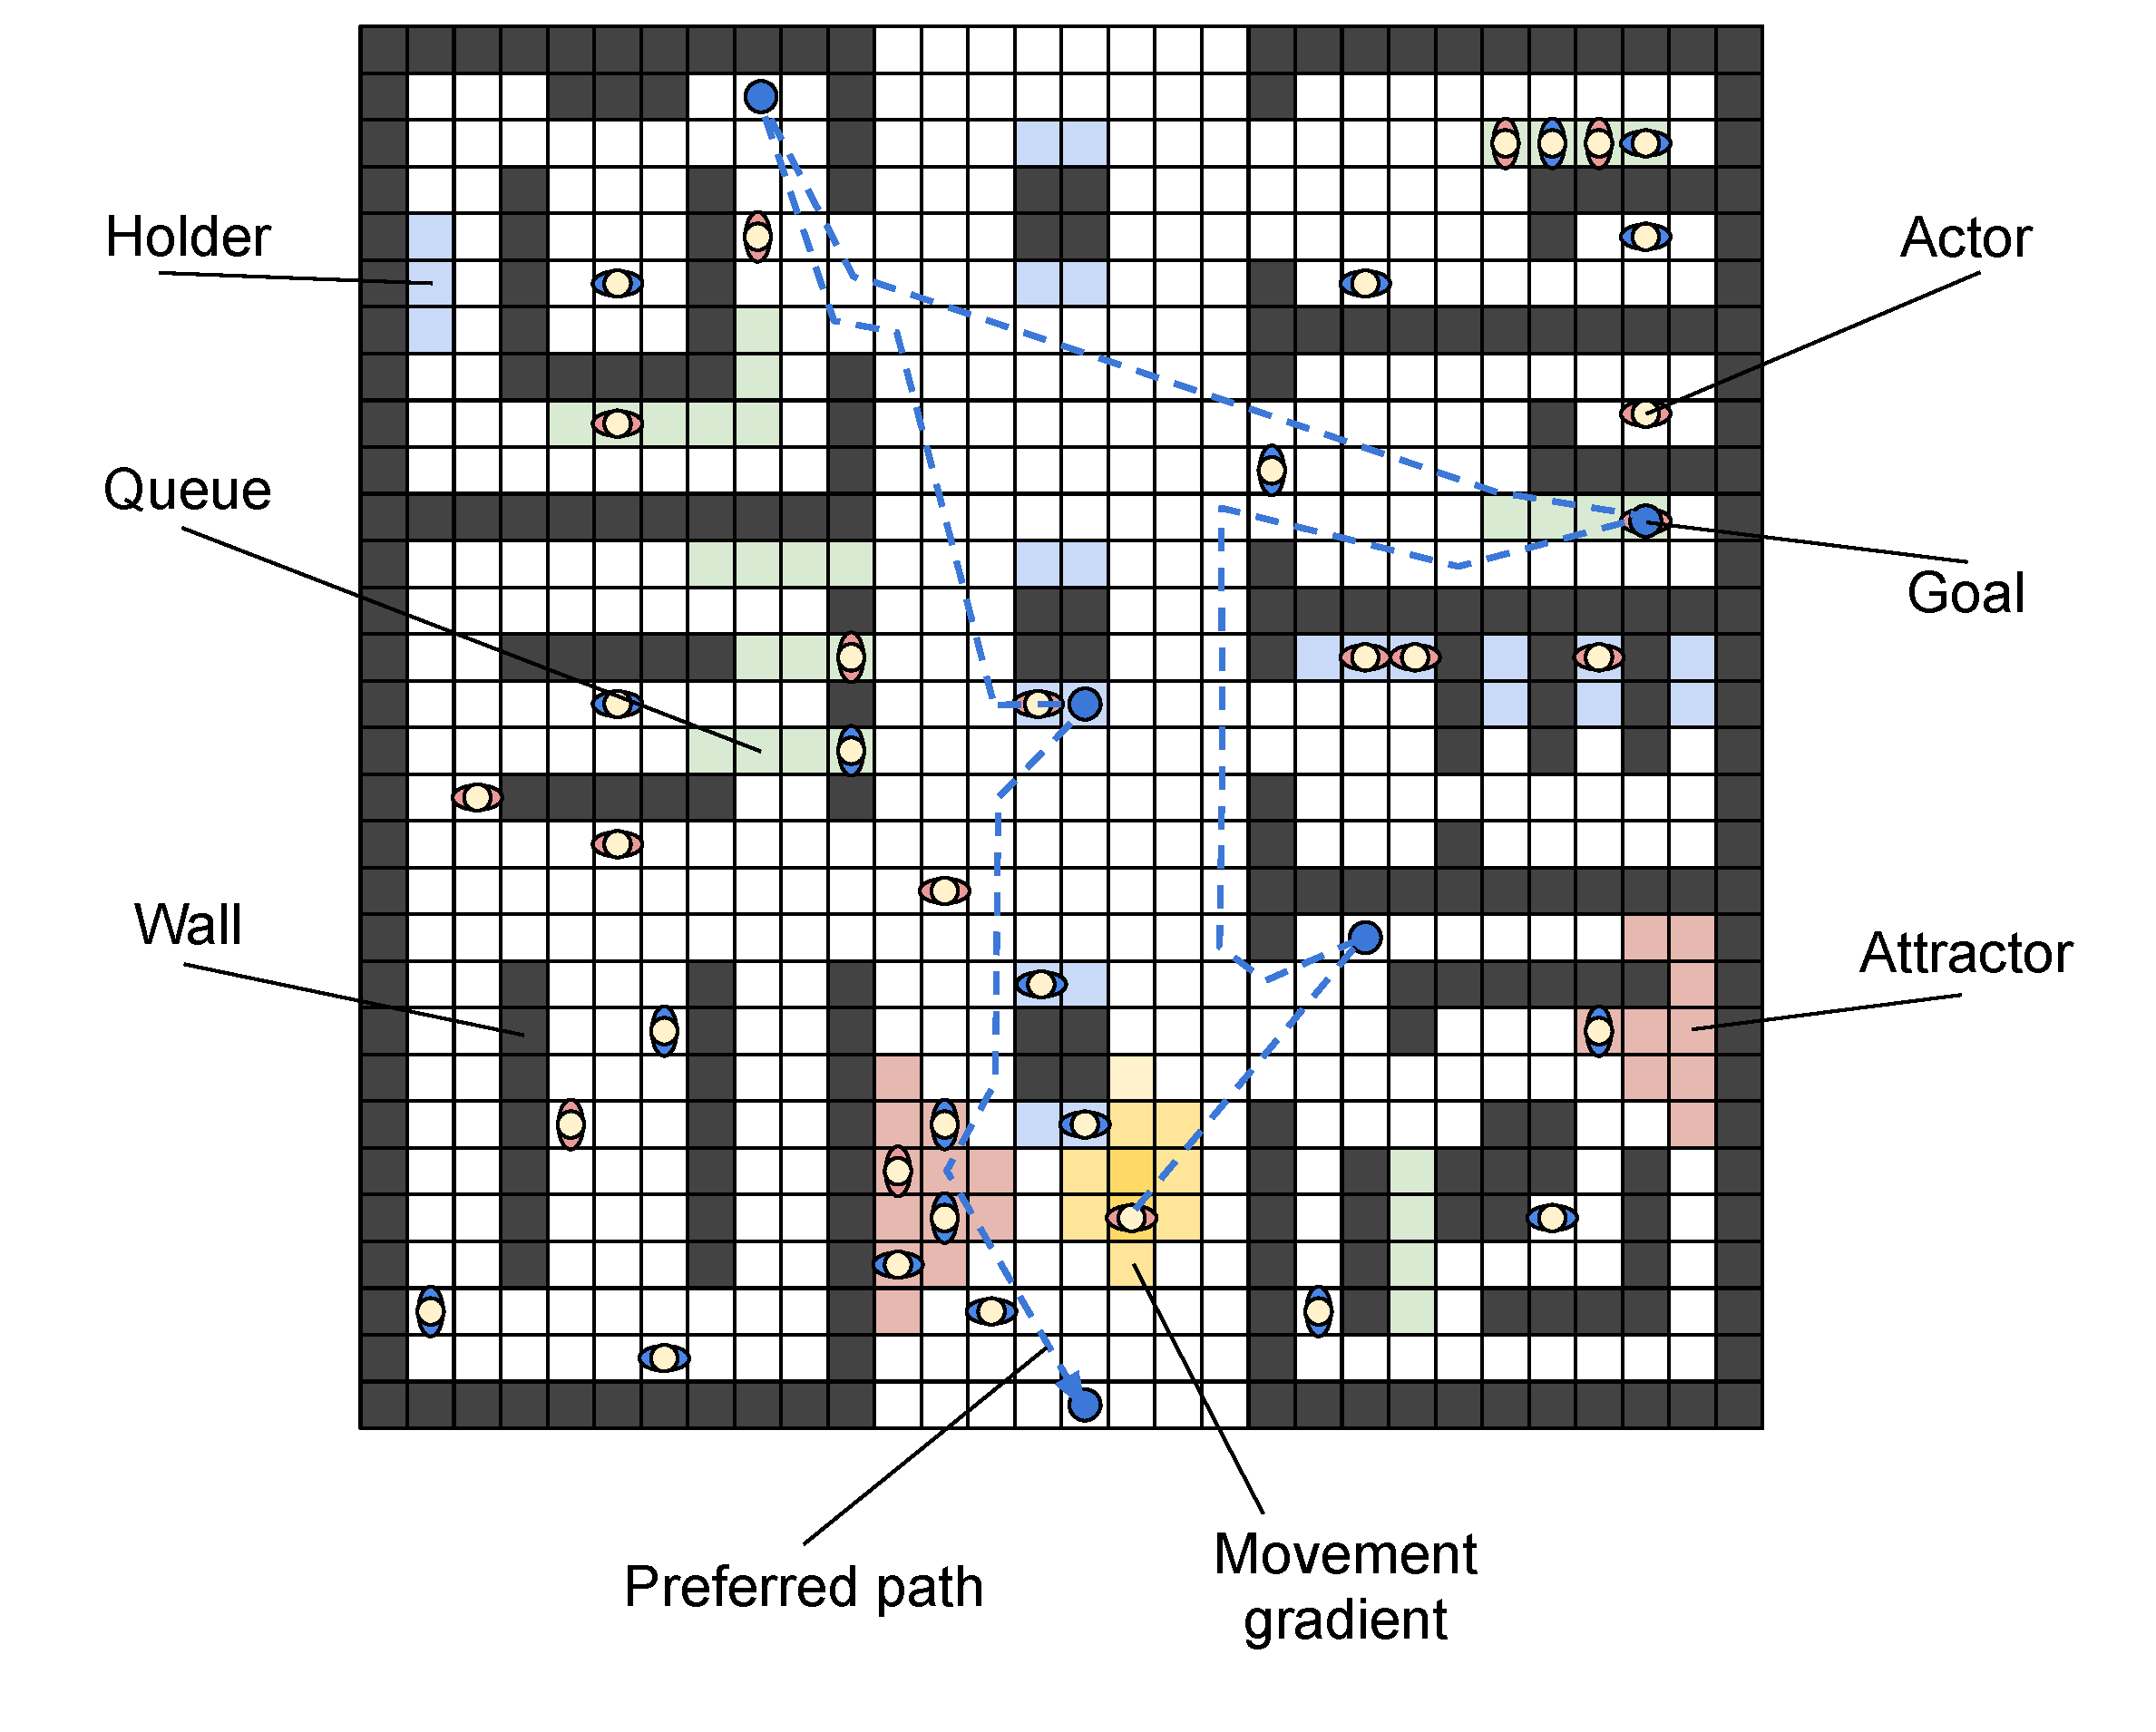
\includegraphics[scale=0.3]{./img/Overview.pdf}
        \caption{Zastosowana dekompozycja problemu.}
        \label{fig:overview}
    \end{figure}

Model centrum handlowego przewiduje istnienie specjalnych stref, wewnątrz których algorytmy odpowiedzialne za poruszanie agentów są modyfikowane lub zastępowane celem modelowanie dobrze zdefiniowanych elementarnych zachowań, takich jak \textit{kolejkowanie}, czy \textit{grupowanie się}.

    % TODO Opis poszczególnych stref.

    \subsection{Atraktory}
    \label{sec:attractors}

    \subsection{Kolejki}
    \label{sec:queues}

    \subsection{Wejścia/wyjścia/przejścia}
    \label{sec:entrance-exits}

    \subsection{Miejsca wstrzymania}
    \label{sec:holders}

\newpage
    \section{Model ruchu ludzi}
    \label{sec:move-model}

\noindent
W zastosowanym algorytmie można wyszczególnieć dwie główne, wzajemnie od siebie zależne fazy - fazę \hyperref[sec:tactical]{taktyczną} oraz fazę \hyperref[sec:operational]{operacyjną}, których interakcję przestawiono na poniższym, uproszczonym diagramie.

    \begin{figure}[h!]
        \centering
        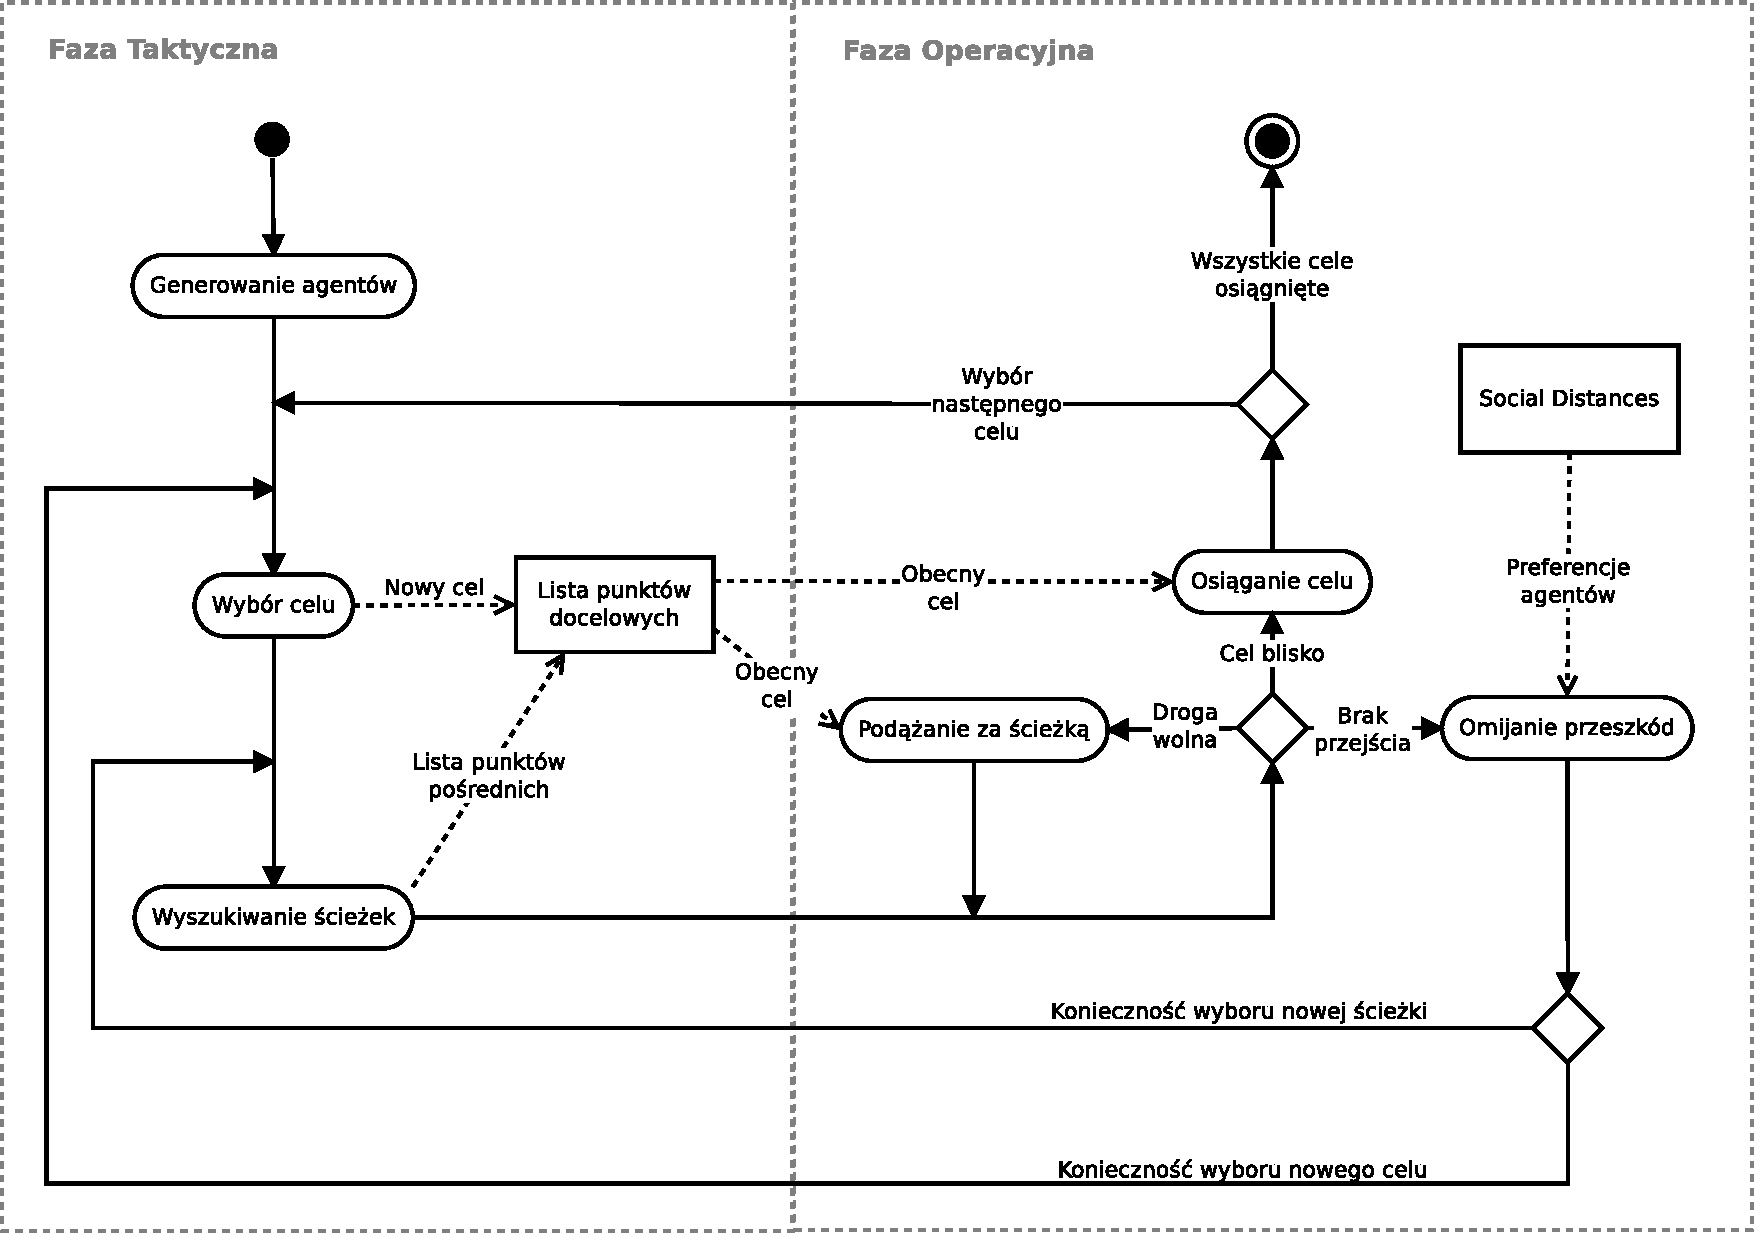
\includegraphics[scale=0.7]{./img/ActorActivity.pdf}
        \caption{Diagram aktywności aktorów.}
        \label{fig:actor-activity}
    \end{figure}

    % TODO Więcej szczegółów na temat generowania aktora i zestawu jego parametrów.
    % TODO Więcej szczegółów na temat algorytmu wybierania miejsc docelonych.

Algorytm rozpoczyna pracę od wygenerowania aktora na podstawie wcześniej zdefiniowanych archetypów.
Dla każdego aktora wybierana jest wstępna lista miejsc docelowych, które zostaną przez niego odwiedzone w cziasie działania symulacji, oraz obliczana jest optymalna ścieżka wiodące do pierwszego wybranego w poprzednim kroku miejsca docelowego. Algorytm następnie modyfikuje ścieżkę w oparciu o mapę rozkładu stref specjalnych centrum handlowego by lepiej modelować faktyczne zamiary danego aktora.

Po wygenerowaniu niezbędnych danych taktycznych dla każdego aktora algorytm przechodzi do fazy operacyjnej, która odpowiada za właściwy ruch aktorów. Faza ta zachodzi w lokalnym otoczeniu każdego agenta i odpowiada za zachowania takie jak omijanie przeszkód, grupowanie się, podążanie za ścieżką i inne akcje związane ze specjalnymi strefami centrum handlowego.
Algorytm na podstawie bezpośredniego otoczenia aktora oraz metadanych dotyczących obecnego celu jego podróży podejmuje decyzje o możliwości wykonania ruchu, lub w przypadku skrajnym o modyfikacji wybranej ścieżki prowadzącej do celu, czy nawet modyfikacji aktualnego celu podróży.
W przypadku osiągnięcia miejsca docelowego algorytm przechodzi do rozpatrywania następnego miejsca docelowego, lub w tryb ``błądzenia'', gdy osiągnięto ostatni cel.

\newpage
        \subsection{Faza taktyczna}
        \label{sec:tactical}

        \begin{figure}[h!]
            \centering
            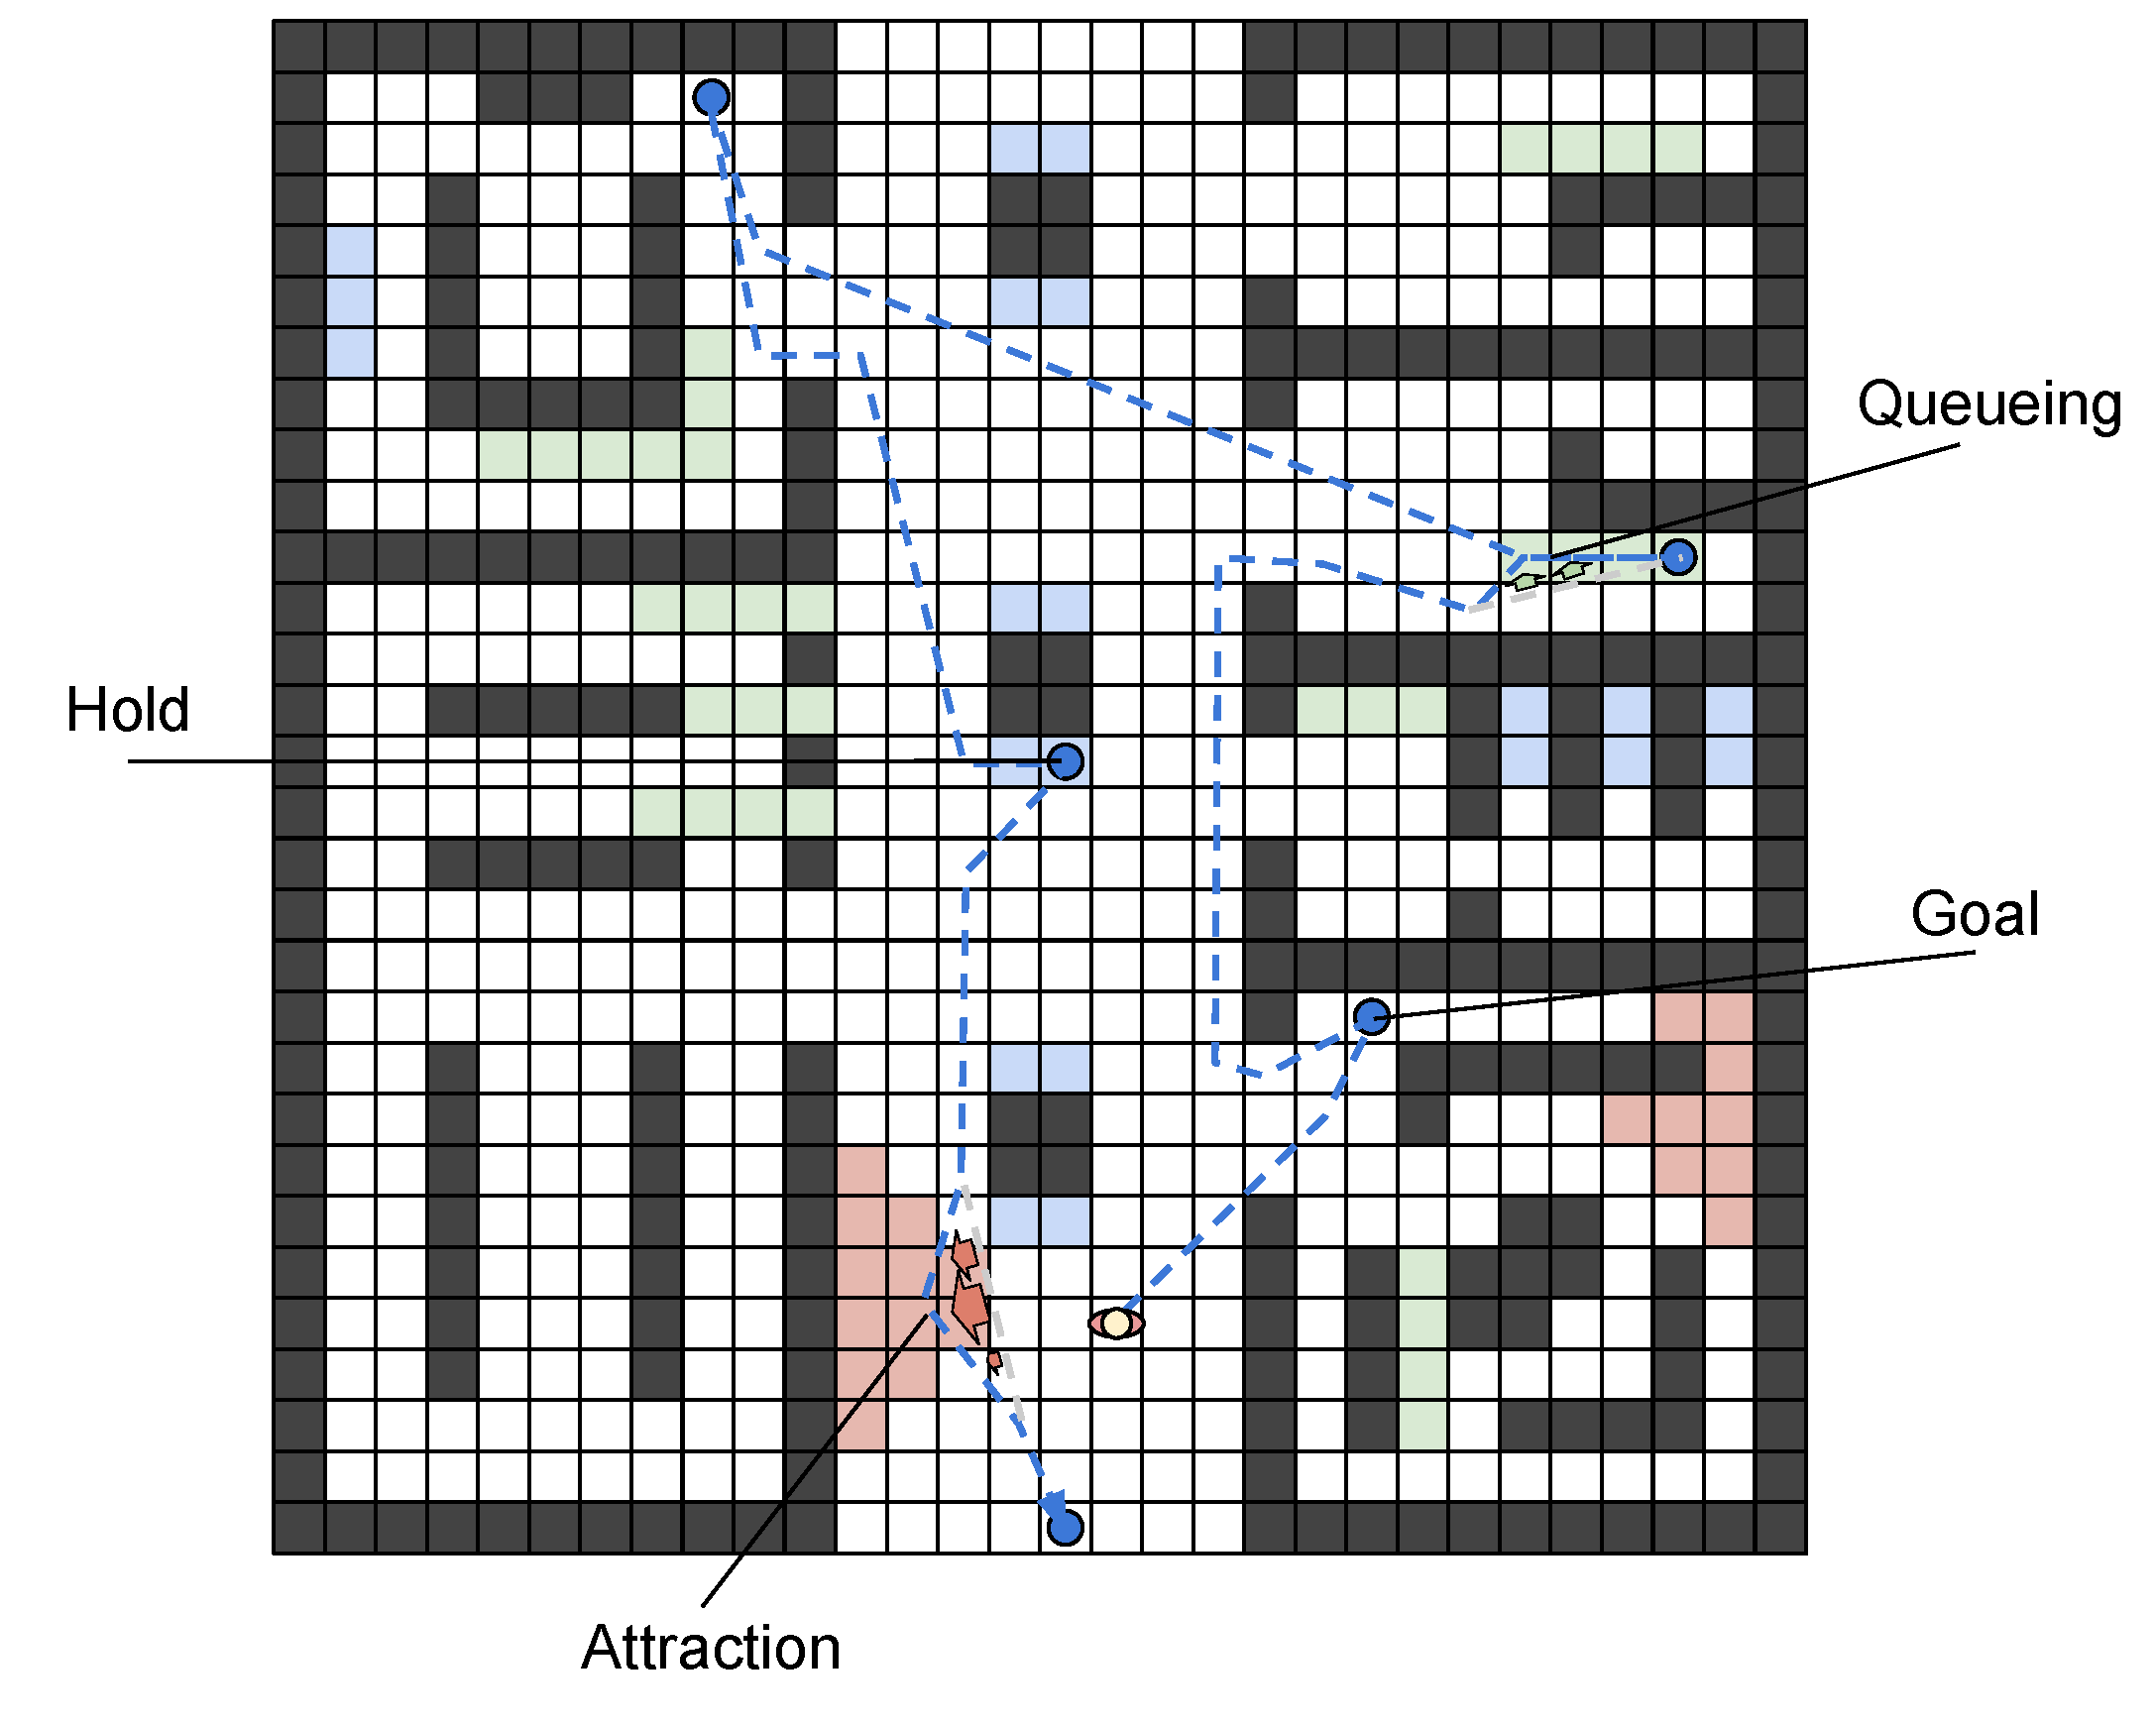
\includegraphics[scale=0.3]{./img/Tactical.pdf}
            \caption{Zakres operacji taktycznej części modelu ruchu.}
            \label{fig:tactical}
        \end{figure}

        % TODO Linki do opisu atraktorów, kolejek itd.

\noindent
Faza taktyczna zachodzi globalnie dla każdego aktora bez uwzględnienia jego lokalnego otoczenia, innych aktorów, czy technicznych właściwości centrum handlowego - nie jest istotnym, czy dany korytarz został zablokowany przez grupę ludzi i nie umożliwia przejścia. Faza ta modeluje abstrakcyjne zamiary aktora i jej celem jest przede wszystkim wybór listy miejsc docelowych oraz wyznaczenie dróg do nich prowadzących, co zostało osiągnięte dzięki \hyperref[sec:path-finding]{algorytmowi znajdowania ścieżek} oraz \hyperref[sec:mall-impl]{mapie rozkładu stref specjalnych} centrum handlowego. Pod uwagę brane są \hyperref[sec:attractors]{atraktory}, \hyperref[sec:queues]{kolejki} i \hyperref[sec:entrance-exits]{schody}, które algorytm stara się osiągnąć modyfikując wcześniej wyznaczoną, optymalną ścieżkę prowadzącą do aktualnego celu podróży.

        \subsection{Faza operacyjna}
        \label{sec:operational}

        \begin{figure}[h!]
            \centering
            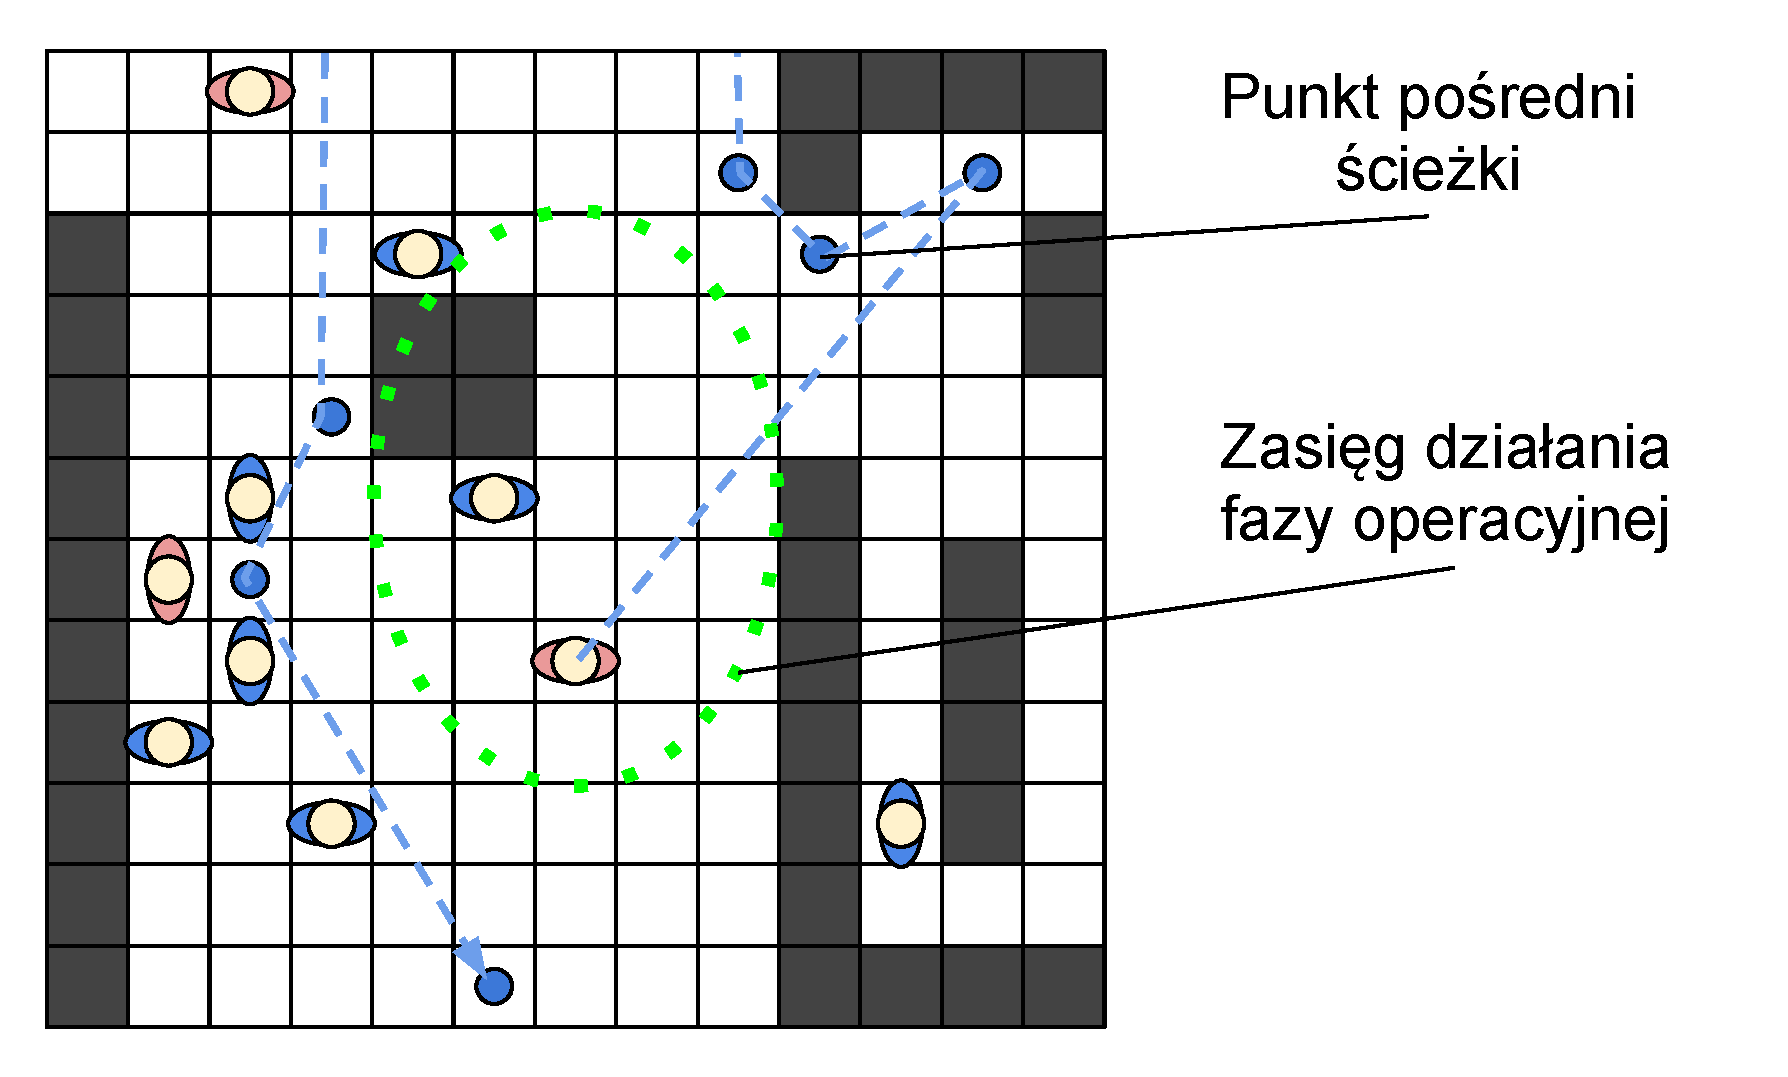
\includegraphics[scale=0.3]{./img/Operative.pdf}
            \caption{Zakres działania operacyjnej części modelu ruchu.}
            \label{fig:operational}
        \end{figure}

        % TODO Potrzeba większego opisu, który bardziej zagłębia się w wybrany algorytm operacyjny.

\noindent
Faza operacyjna zachodzi w lokalnym otoczeniu każdego aktora, a jej celem jest wykonanie właściwego ruchu aktora. Faza ta jest odpowiedzialna za unikanie kolizji i omijanie przeszkód. Pod uwagę brani są inni aktorzy oraz metadane dotyczące drogi prowadzącej do aktualnego celu podróży wygenerowane w taktyczniej fazie działania algorytmu.

\newpage
    \section{Implementacja}
    \label{sec:implementation}

     % TODO Trzeba zweryfikować i opisać technikalia implementacji...
     % TODO Ofkors po uprzednim zaimplementowaniu całości ;)

        \subsection{Reprezentacja centrum handlowego}
        \label{sec:mall-impl}

        \begin{figure}[h!]
            \centering
            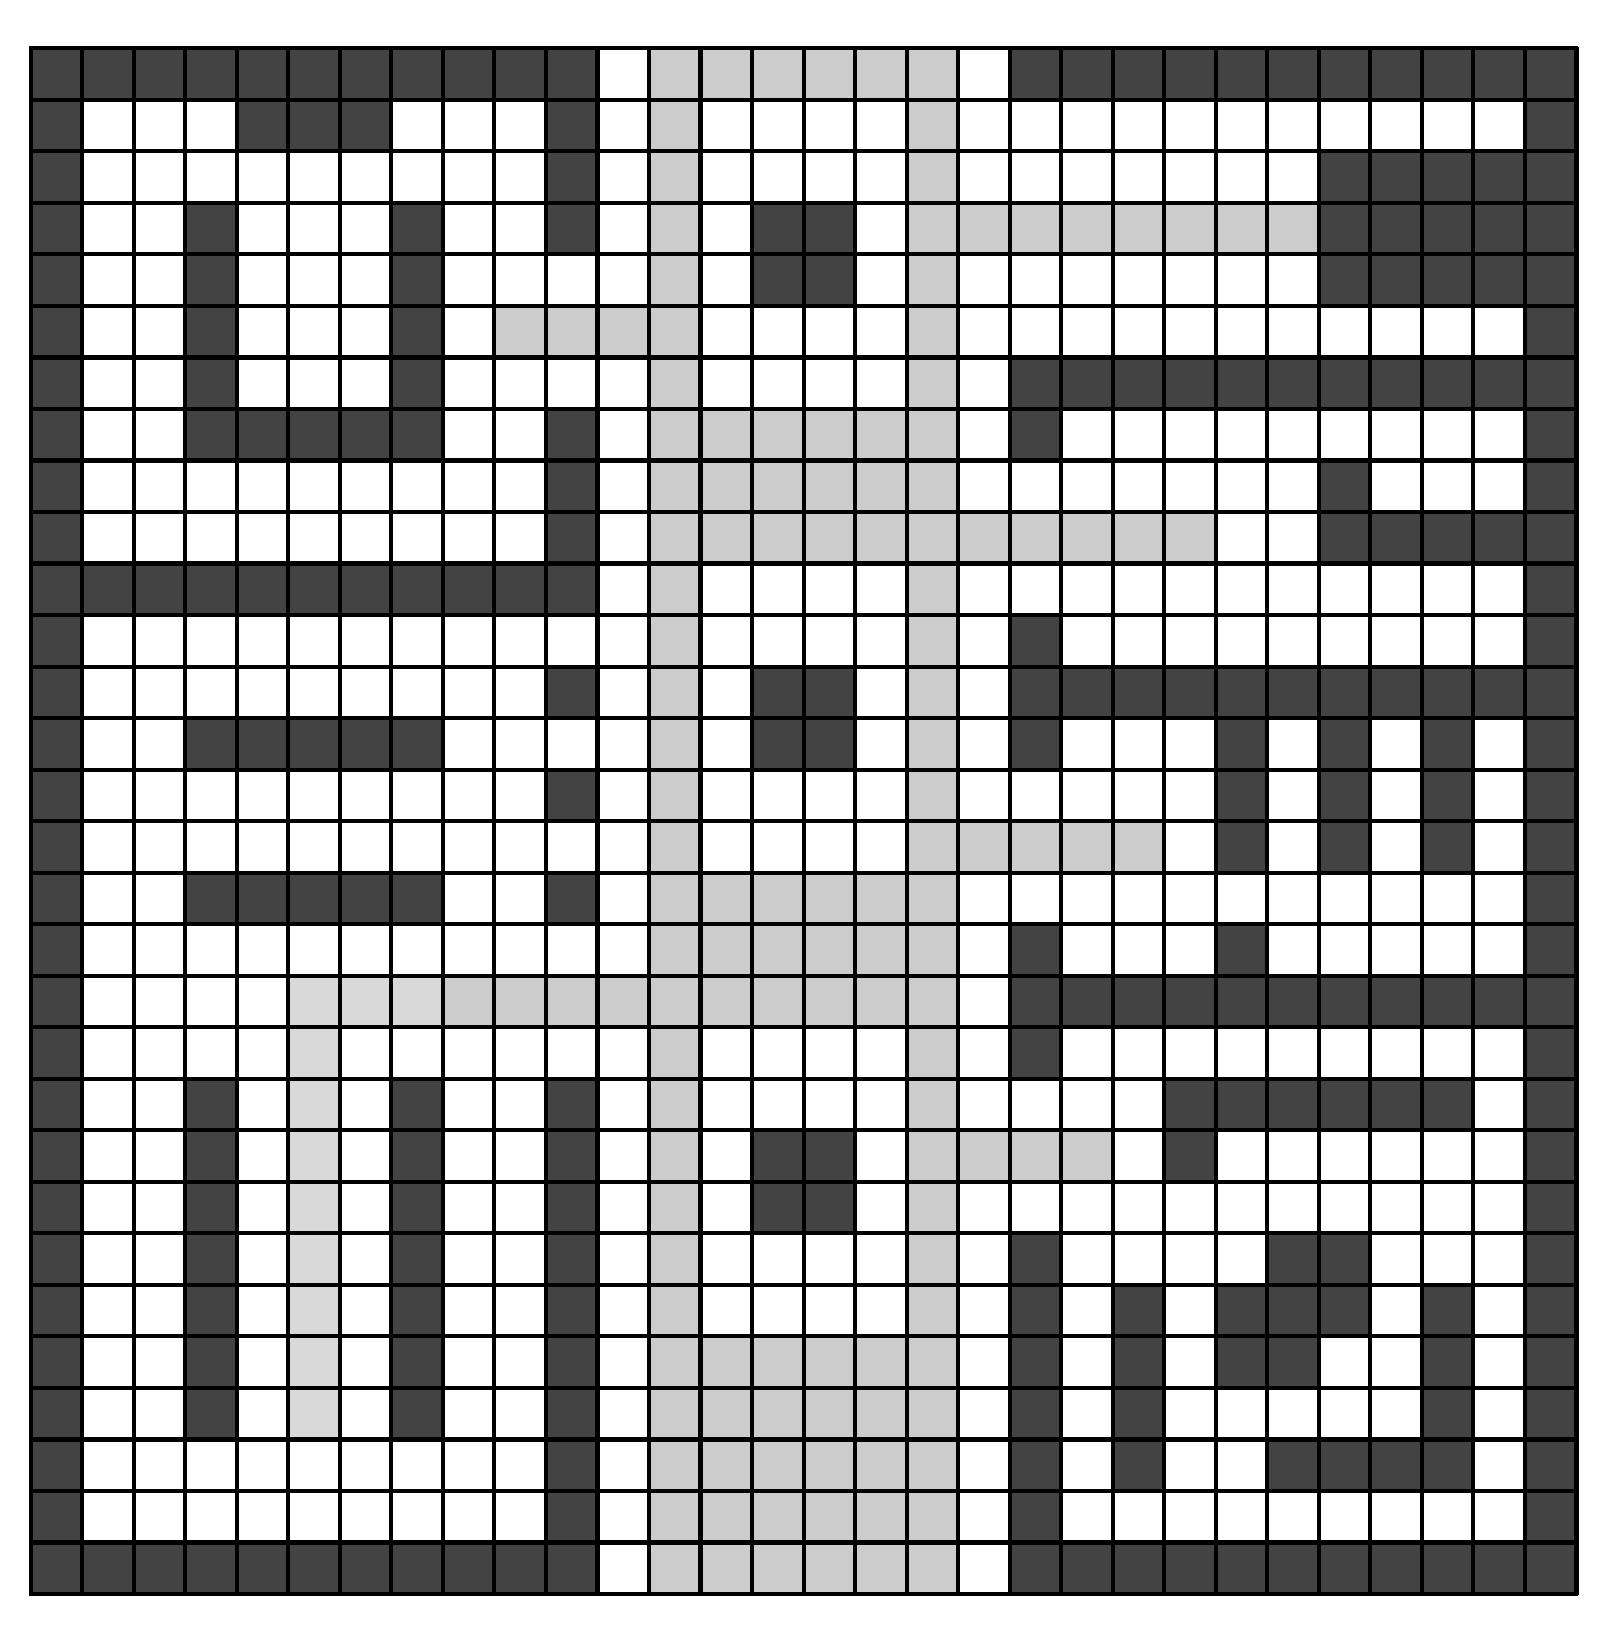
\includegraphics[scale=0.2]{./img/MallLayout.pdf}
            \caption{Przykładowy rozkład pomieszczeń małego centrum handlowego.}
            \label{fig:mall-layout}
        \end{figure}

        \begin{figure}[h!]
            \centering
            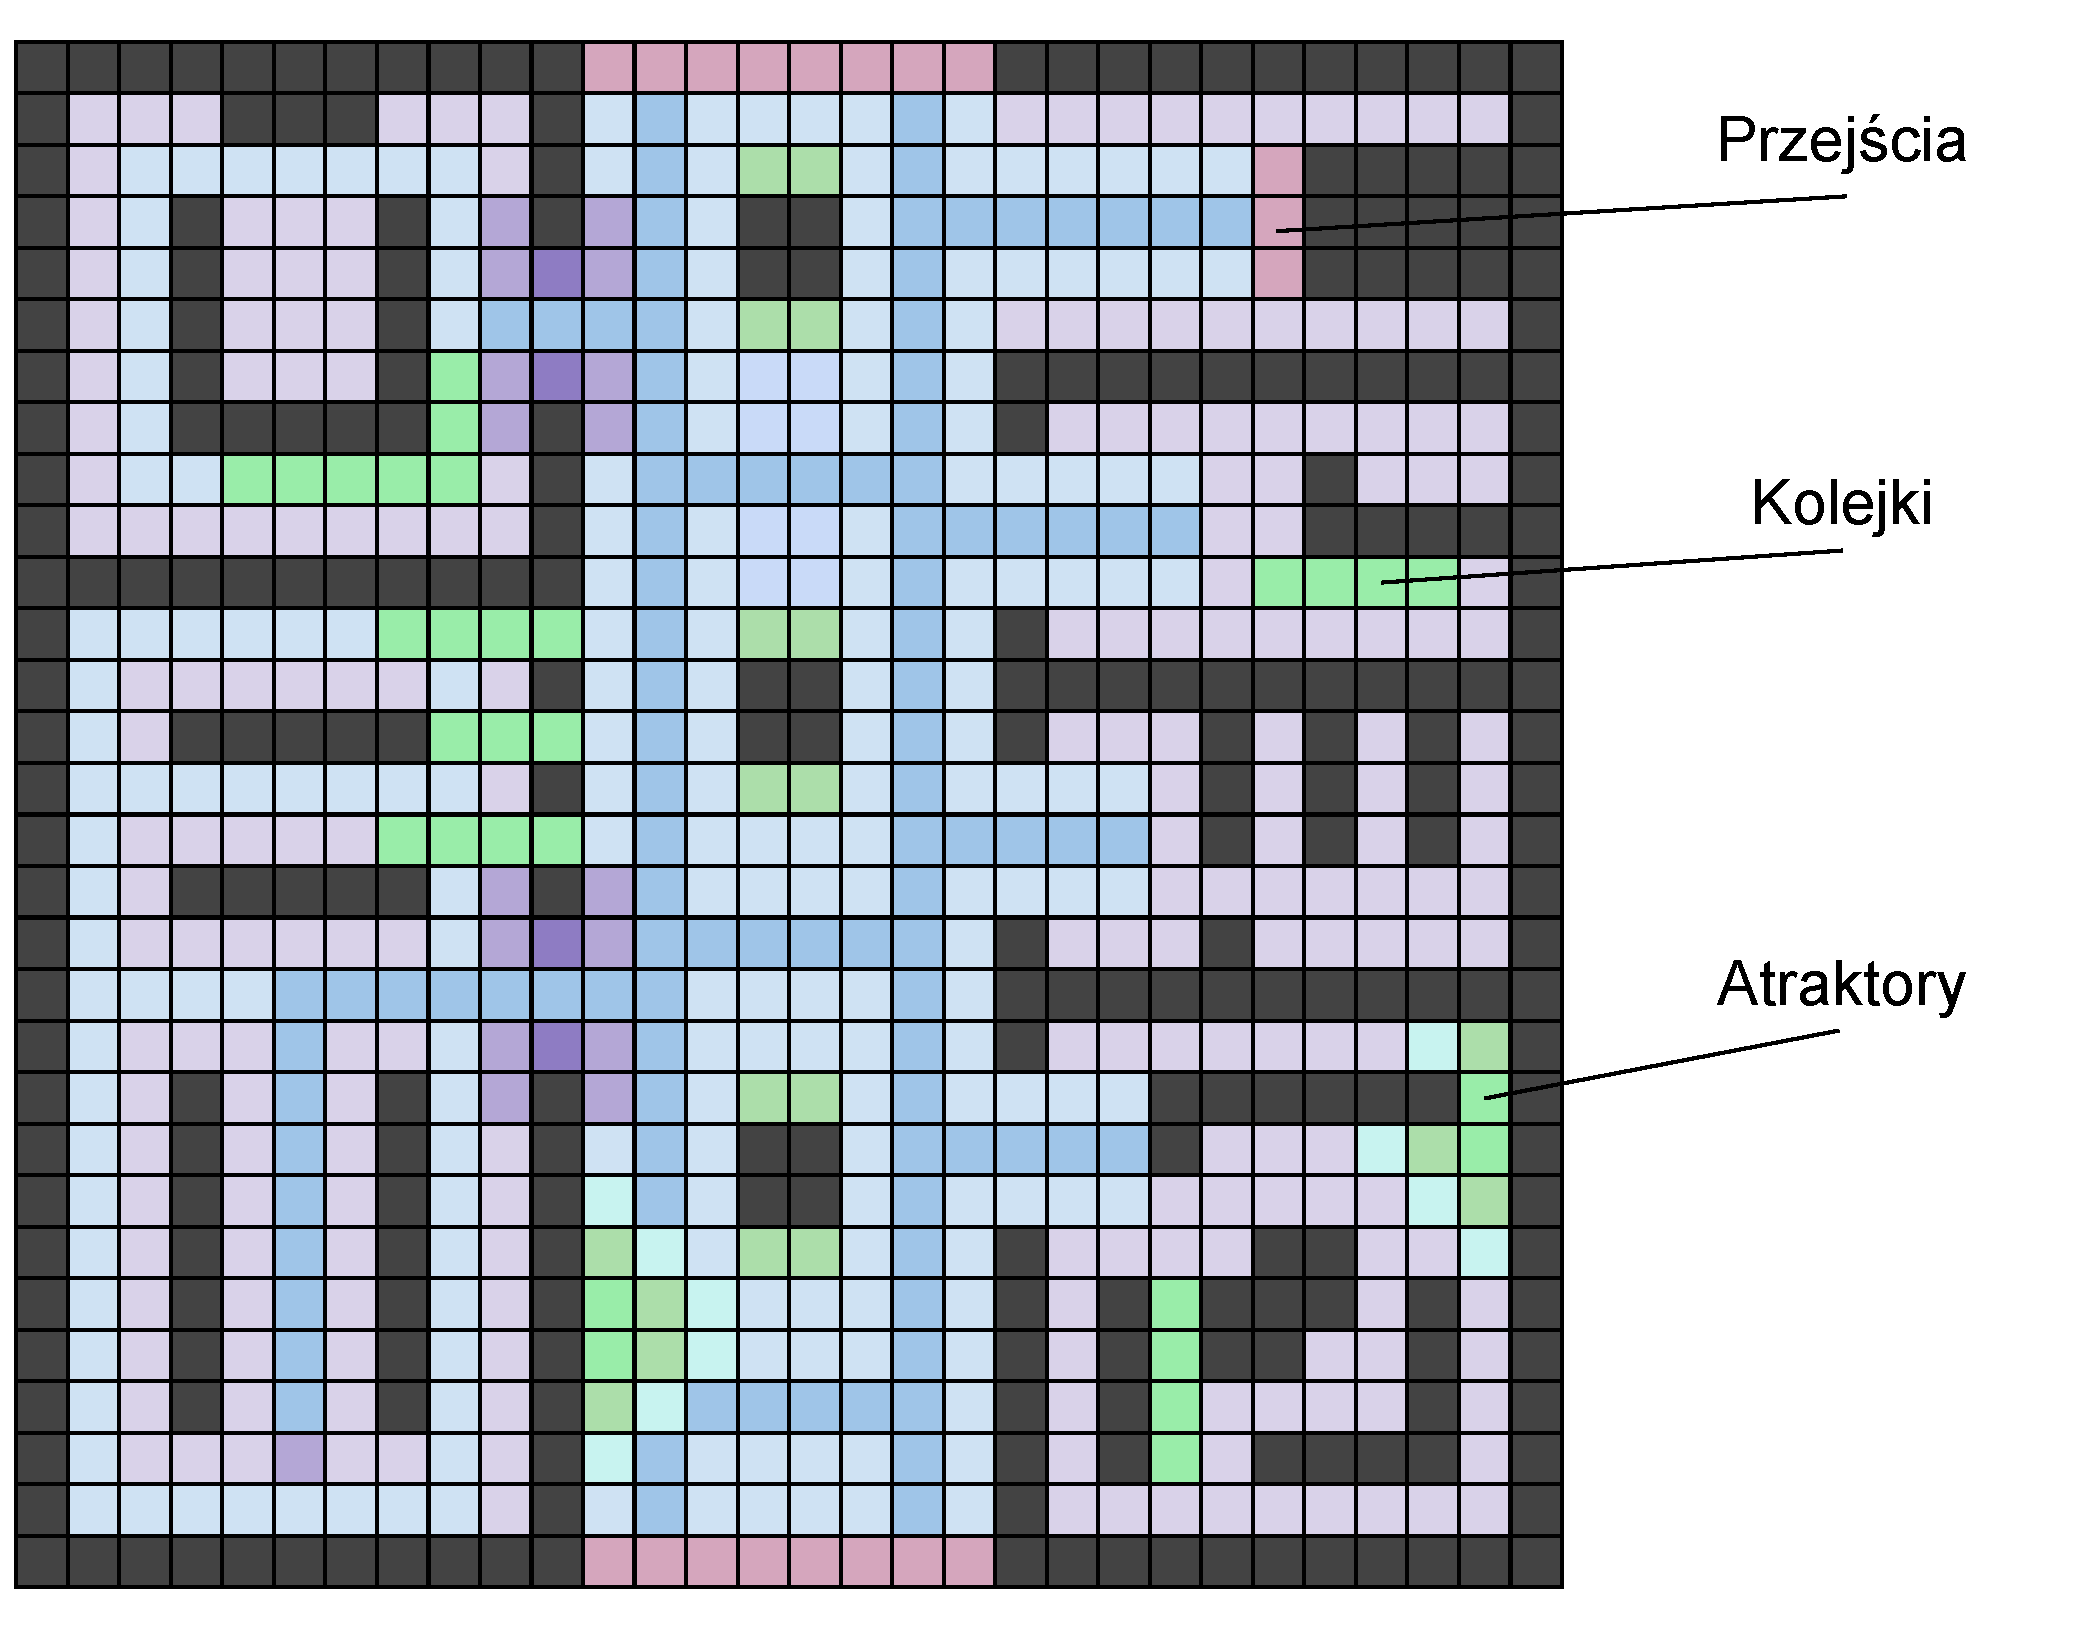
\includegraphics[scale=0.2]{./img/MallFeatures.pdf}
            \caption{Przykładowy rozkład stref specjalnych małego centrum handlowego.}
            \label{fig:mall-features}
        \end{figure}

        % TODO Opisać jak obsługiwane są wielopiętrowe centra handlowe.
        % TODO Opisać, jak kodowane są poszczególne strefy specjale.

        \subsection{Reprezentacja agentów}
        \label{sec:actor-impl}

        % TODO Opisać algorytm A*

        \subsection{Znajdowanie ścieżek}
        \label{sec:path-finding}

        % TODO Opisać algorytm A*

\newpage
    \section{Symulacja i analiza wyników}
    \label{sec:sota}

    % TODO Zasymulawać, zebrać dane i je przeanalizować porównując do danych rzeczywistych.

\newpage
    \section{Referencje}
    \label{sec:refs}

    % TODO Trzeba znaleźć sposób, by linkować bezpośrednio do konkretnych pozycji na liście, nie do całej listy.

    \begin{itemize}
        % TODO Trzeba wybrać jedną do dwóch publikacji, które zgrabnie opisują model Social Distances.
        \begin{item} \label{refs:social-distances-1} Social Distances \end{item}
        \item Rzeczy z sec:intro...
        \item Rzeczy z sec:sota...
        \item Rzeczy z sec:tactical...
        \item Rzeczy z sec:operational...
        \item \ldots
    \end{itemize}
\end{document}
